%\documentclass[10pt,oneside,twocolumn,letterpaper]{article}
%\documentclass[12pt,oneside,onecolumn,letterpaper]{article}
\documentclass[12pt,twoside,onecolumn,letterpaper]{article}
%\documentclass[10pt,oneside,onecolumn,letterpaper]{article}
\usepackage[spanish]{babel}
\usepackage[utf8]{inputenc}
\usepackage{hyperref}
\usepackage{graphicx}
\usepackage{fancyhdr}
\usepackage{enumerate}
\usepackage{color}
\usepackage{colortbl}
\definecolor{gray}{cmyk}{0.0,0.0,0.0,0.60}
 
\hoffset-25mm
\voffset-25mm
%\marginparwidth=0mm
%\marginparsep=0mm
\headheight=16pt
\oddsidemargin=25mm
\evensidemargin=25mm
\textwidth=165mm
\topmargin=20mm
\textheight=220mm

\pagestyle{fancy}
\fancyhf{}
\fancyhead[RO]{\small{\textcolor{gray}{\textsc{Propuesta de investgaci\'on: Locomoci\'on b\'ipeda ...}}}}
\fancyhead[LO]{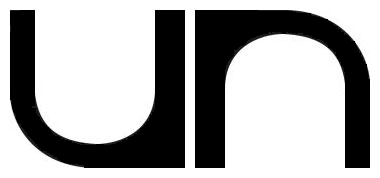
\includegraphics[scale=0.05]{../images/unlogo.png}}
\fancyhead[LE]{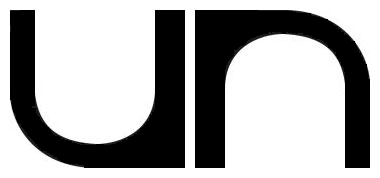
\includegraphics[scale=0.05]{../images/unlogo.png} \small{\textcolor{gray}{\textsc{Doctorado en ingenieria: Mecanica y Mecatronica}}}}
\fancyfoot[CO,CE]{\thepage}
\fancyfoot[LO,RE]{\scriptsize{\textcolor{gray}{\emph{Version 0.4}}}}

\title{
\includegraphics[scale=0.15]{../images/unescudobn.png}\\\vspace{-0.2cm}
  \textsc{\underline{\small{Universidad Nacional de Colombia}}\\\tiny{Sede Bogot\'a}\\\small{Facultad de Ingenier\'ia\\\vspace{-0.2cm}Unidad de Posgrado}}\\\vspace{0.5cm}
       \LARGE \textbf{Locomoci\'on de caminadores b\'ipedos: Rob\'otica subactuada, control, dise\~no y aplicaciones}}
\author{J.A. Castillo Le\'on \thanks{jacastillol@unal.edu.co}}
\date{}
\begin{document}

\renewcommand{\tablename}{Tabla}

\maketitle
{\large\textbf{Director de investigaci\'on:} PhD. Ing. Ricardo Ram\'irez Heredia}\par\vspace{0.7cm}
{\large\textbf{L\'inea de investigaci\'on:} Rob\'otica}
\section{Justificaci\'on}
\label{sec:justify}
Buscando una proliferaci\'on robusta de la rob\'otica en el pa\'is a nivel tecnol\'ogico y del conocimiento de esta \'area, se da acontinuaci\'on la justificaci\'on de este proyecto de investigaci\'on, propuesta que se ve acotada a ser trabajada en el mundo de la r\'obotica de caminadores.  Las tendencias a nivel mundial que se desarrollan en este tema actu\'almente, crecen cada d\'ia a pasos agigantados provocados por cientos de grupos de investigaci\'on pertenecientes a Universidades, Institutos, Centros y Laboratorios en todo el mundo.\par
Aunque la Universidad Nacional de Colombia ya comenz\'o sus investigaciones en el \'area con interesantes resultados\cite{M2005,M2005a,Roa2006,Heredia2007}, en donde se han construido lazos por medio de investigadores, profesores y estudiantes de la Universidad con otros grupos de vital importancia a nivel mundial en el \'area, como es el caso de \cite{Englsberger2011,Ott2011,M2013}. Desde hace unos siete a\~nos no se han desarrollado proyectos importantes en el \'area de caminadores.\par
El campo de la rob\'otica b\'ipeda ha superado algunos problemas y han surgido unos nuevos, en donde las soluciones encontradas han sido generadas integrando m\'ultiples fuentes de conocimiento, en \'areas como: los sistemas embebidos\cite{Barker2010,Pan2010,Kimm2012,Wang2011,Amir2013}, la biomec\'anica\cite{Mahmoodi2013,Lim2014,Wu2013,Aoustin2013,Chiang2013,Xiang2010,Hobon2014}, el modelado de sistemas mec\'anicos\cite{Chiang2013}, la s\'intesis de mecanismos\cite{Li2008,Aoustin2013,Wu2013a,Xu2013,Hobon2014}, la optimizaci\'on\cite{Xiang2010,Lim2014,Kherici2014,Mahmoodabadi2014}, la computaci\'on flexible\cite{Wang2013,Kherici2014,Mahmoodabadi2014}, la inteligencia artificial\cite{Treesatayapun2014,Yuan2014,Wu2014,Wang2013} y el control\cite{Dou2013,Treesatayapun2014,Yuan2014,Wu2014}.\par
A continuaci\'on se organizan algunos aspectos que forman parte de la justificaci\'on:
\begin{itemize}
\item Dise\~nos de caminadores de bajo costo, funcionales, did\'acticos, modulares y de prototipado r\'apido especiales para la ense\~nanza de la rob\'otica, el control y los sistemas distribuidos, y la comprobaci\'on de teor\'ias de control de varias capas de locomoci\'on.
\item Inter\'es personal por el tema, ya que despierta toda mi curiosidad y me apasiona, es un \'area en la que aplica la Mecatr\'onica en todo su poder. Involucrando la electr\'onica, la mec\'anica, la teor\'ia de la computaci\'on, la programaci\'on y su experimento debe resultar en algo \'util y real\cite{Castillo2007,Castillo2008,Castillo2010}.
\item \emph{Aplicabilidad:} La aplicaci\'on de los conocimientos que se obtengan servir\'an la soluci\'on de problemas y productos en \'areas como: la industria de los manipuladores en el \'area de la teleoperaci\'on\cite{Treesatayapun2014,M2013}, la manufactura en el transporte de materiales y ensambles\cite{Roy2013}, la fabricaci\'on de pr\'otesis\cite{Roa2006}, la fisioterapia\cite{Kang2013}, la educaci\'on como herramienta did\'actica y motivacionial\cite{Ishida2004}, el entretenimiento,el area de la teor\'ia de juegos y agentes inteligenes como es el caso del futbol de robots\cite{Ishida2004}.
\item \emph{Viabilidad:} El proyecto y la Universidad cuenta con: 
  \begin{enumerate}[1)]
  \item Recursos f\'isicos como centros de mecanizado, impresoras 3D, salas CAD con herramientas computacionales como: Matlab, Ansys, SolidWorks, plataformas rob\'oticas.
  \item Profesores, grupos de investigaci\'on y materias bien formadas en temas pertinentes para esta investigaci\'on como Rob\'otica, Biomec\'anica, Sistemas Embebidos, Control Avanzado, Computaci\'on Flexible, Aprendizaje de m\'aquina, Inteligencia Artificial, Optimizaci\'on, Manufactura Computalizada, Redes de comunicaci\'on y otras m\'as.
  \item  Mecanismos y concursos internos y externos para obtener recursos econ\'omicos para fabricaci\'on de prototipos, sensores, actuadores, herramientas, materiales e insumos.
  \item Posibles lazos con importantes grupos de investigaci\'on e investigadores como Justin DLR(por medio de PhD Maximo Roa), Robonaut 2 GM-NASA(por medio de PhD. Leandro Barajas).
  \item Experiencia del director de investigaci\'on de esta propuesta con aproximadamente 20 a\~nos de experiencia, con trabajos en el tema como \'articulos\cite{Heredia2007}, cap\'itulos de libros\cite{M2005,M2005a}, direcciones de tesis de pregrado y posgrado, y materias de pregrado y posgrado en la Universidad.
  \item Experiencia y perfil del investigador en el tema de este proyecto, con 8 a\~nos de experiencia en temas de rob\'otica serial y paralela, con trabajos como: direcci\'on de tesis de pregrado\cite{Cortes2009,Valencia2009,Barragan2009,Silva2009}, art\'iculos\cite{Castillo2007}, librer\'ias\cite{Castillo2008} y software de simulaci\'on\cite{Castillo2010}, y la materia de pregrado de Rob\'otica en la Universidad Nacional de Colombia durante tres a\~nos y medio consecutivos. Adem\'as de experiencia en temas de automatizaci\'on, control e instrumentaci\'on en la industria y la academia.
  \end{enumerate}
\end{itemize}

\section{Objetivo general y objetivos espec\'ificos}
\label{sec:objs}

\subsection{Objetivo general}
\label{sec:objgen}
El principal objetivo de esta investigaci\'on se describe de forma global y gr\'afica en la Figura \ref{fig:objGen}, y es enunciado a continuaci\'on:\par
\textbf{OG:} Dise\~nar y construir un \emph{marco de experimentaci\'on}\footnote{compuesto por el dise\~no de una red de sensores-actuadores distribuida y un conjunto de dise\~no de eslanbones y articulaciones modulares para frabricados mediante prototipado r\'apido} mediante el cual se pueda implementar\footnote{estudiar, proponer y/o comprobar} las hip\'otesis que solucionen los problemas de locomoci\'on de la rob\'otica subactuada y de caminadores\footnote{que permita la b\'usqueda de estructuras mecatr\'onicas eficientes energ\'eticamente, capaces de lograr la locomoci\'on requerida por las necesidades fundamentales de los robots caminadores}.\par
\begin{figure}[!htb]
  \centering
  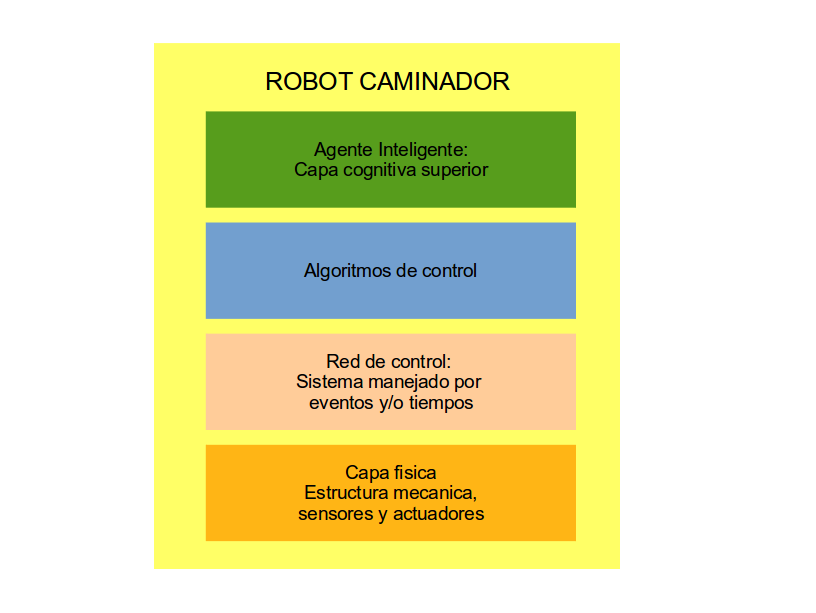
\includegraphics[scale=0.5]{../images/objGen.png}
  \caption{Objetivo General}
  \label{fig:objGen}
\end{figure}

\subsection{Objetivos espec\'ificos}
\label{sec:objesp}
\begin{enumerate}[\textbf{OE:} 1.]
\item Modelar, simular, analizar y sintetizar mecanismos subactuados que optimicen la energ\'ia para la locomoci\'on de caminar, saltar o correr.\par 
\item Dise\~nar y construir una plataforma rob\'otica modular modular y para prototipado (ver Figura \ref{fig:objCapas} Capa Física), capaz de configurar cadenas cinem\'aticas  controladas y/o monitoreadas bajo el sistema distribuido.\par
\item Implementar un sistema distribuido de sensores y actuadores que funcione en tiempo-real  (ver Figura \ref{fig:objCapas} Capa de sensorial y de Actuaci\'on), bajo el principio de manejo por disparo-de-eventos y/o manejo por disparo-por-tiempos\cite{Kimm2012}.\par
\item Dise\~nar, simular e implementar diferentes controles de locomoci\'on (ver Figura \ref{fig:objCapas} Capa de control de locomoci\'on) inspirados en las nuevas tendencias de investigaci\'on de caminadores sobre plataformas rob\'oticas modulares construidas.\par
\item Dise\~nar, simular e implementar estrategias y actividades colaborativas usando una red de caminadores  (ver Figura \ref{fig:objCapas} Capa Cognitiva.).\par
\end{enumerate}
\begin{figure}[!htb]
  \centering
  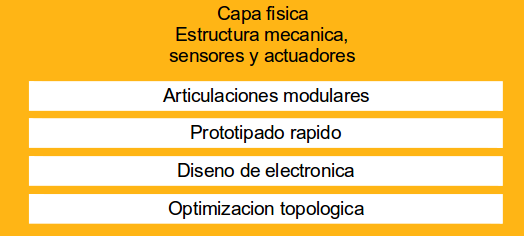
\includegraphics[scale=0.45]{../images/objCapaFisica.png}
  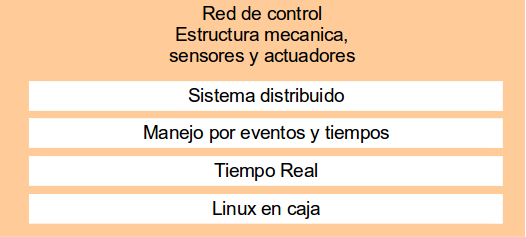
\includegraphics[scale=0.45]{../images/objCapaRAS.png}\\
  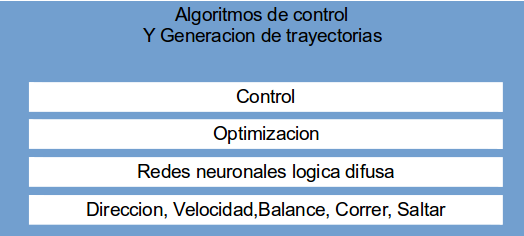
\includegraphics[scale=0.45]{../images/objCapaControl.png}
  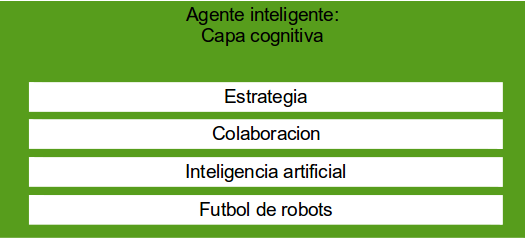
\includegraphics[scale=0.45]{../images/objCapaCognitiva.png}
  \caption{Objetivos Específicos}
  \label{fig:objCapas}
\end{figure}

\section{Estado del arte}
\label{sec:arte}
Revisando la amplia literatura encontrada sobre \emph{la locomoci\'on}, la mayor inquietud citada viene de la Rob\'otica\cite{Xiang2010,Mattar2013} y la Biomec\'anica\cite{Xiang2010,Mattar2013}, \'areas que muestran su interés en replicar las estructuras y/o las funcionalidades de movilidad de diferentes seres vivos\cite{Xu2013,Chiang2013} o como muchos autores\cite{Xu2013} y congresos\cite{RB2009} hacen referencia a \emph{biom\'imesis}. Estas necesidades van desde solo comprobar las leyes f\'isicas sobre un sistema mecatr\'onico\cite{Barker2010,Lens2011} hasta dise\~nar m\'aquinas robotizadas que sirvan al hombre en ambientes de riesgo donde \'este no deber\'ia encontrarse\cite{Seifried2014,Wu2013a}, o desde solo entender la marcha humana para proponer una terap\'ia sobre alg\'un m\'usculo lesionado\cite{Kang2013} hasta el remplazo de una extremidad que mejore la calidad de vida de una persona v\'ictima de alg\'un accidente\cite{Roa2006,Wu2013a}.\par
Dentro de la locomoci\'on b\'ipeda se diferencia dos formas generales del modo de andar: una bajo el r\'egimen de caminata y otra bajo el r\'egimen de correr, trotar o galopar\cite{Geyer2006}. La manera de distinguir estos modos viene dada por las distintas fase que definen un ciclo de andar, la diferencia entre caminar y trotar, ser\'a que durante la caminata habr\'an fases con doble contacto con el piso, mientras que en el r\'egimen de trotar o correr no existirá fases con doble contacto\cite{Geyer2006}, adem\'as en el regim\'en de correr existe una fase en la que no ocurre ningún contacto, fase que se encuentra con el nombre de vuelo.\par
Una de las posibles clasificaciones que se pude hacer en caminadores es seg\'un su tipo de balance durante la caminata, este balance puede ser est\'atico o din\'amico\cite{Braunl2008}. Las mayores inquietudes y retos al d\'ia de hoy se encuentran en el balance din\'amico, pues este tipo de balance se acerca m\'as a una caminata \'optima y natural, como la que han logrado los seres humanos durante toda su evoluci\'on.\par
Otra clasificaci\'on podr\'ia ser los modelos físico, que se han utilizado para describir la caminata\cite{Xiang2010}: 1) modelos de p\'endulo invertido, 2) din\'amica pasiva de la caminata y 3) ZMP punto de momento cero. Una caracter\'istica de los tres modelos f\'isico citados anteriormente, es que sus movimientos son generados en tiempo real\cite{Xiang2010}. En el caso de la din\'amica pasiva de la caminata, recientes tendencias en b\'usqueda de dise\~nos naturales tanto en las estructuras mec\'anicas como en los esquemas de control buscan mejorar los problemas energ\'eticos que resultaron de los mejores avances que se han obtenido en el tema gracias al concepto del ZMP\cite{Xiang2010}.\par
Aunque la caminata pasiva lleva en estudio m\'as de 25 a\~nos, tuvo un momento de oscuridad cuando el ZMP, el cual lleva m\'as de 40 a\~nos, logr\'o resultados tecnol\'ogicos en los a\~nos ochenta\cite{Vukobratovic2004}. Desde hace 25 a\~nos se retomo nuevamente el estudio de la caminata pasiva ya no solo como ejemplo acad\'emico\cite{McGeer1990a}, dando nuevos caminos en el control y acerc\'andose a la soluci\'on desde el punto de vista de la optimizaci\'on de la energ\'ia\cite{Goswami1996}, proponiendo as\'i a la caminata activa la generaci\'on \'optima de trayectorias\cite{Gregg2010}.\par
Los modelo mec\'anicos bio-inspirados se encuentran de dos clases\cite{Xiang2010}. El primero que toma el sistema \'oseo para luego proponer unos actuadores distintos a los músculos\cite{Wang2012} y el segundo que analiza adem\'as del sistema \'oseo, el sistema muscular para tomar los m\'usculos del cuerpo humano como los actuadores del sistema\cite{Kang2013,Roa2006}. Los modelos matem\'aticos de estos modelos bio-inspirados est\'an basados en la din\'amica multicuerpo\cite{Xiang2010}, donde cabe resaltar que los modelos m\'usculo-esquel\'eticos incrementan la carga computacional por el gran n\'umero de grados de libertad\cite{Xiang2010}, mientras que los modelos basados \'unicamente en el sistema oseo son f\'aciles de simplificar y en la mayor\'ia de los casos tan solo se tiene en cuenta las longitudes de las extremidades analizadas reduciendo también un importante n\'umero de grados de libertad\cite{McGeer1990a}. Cabe resaltar de diferentes herramientas y formalismos son empleadas en la literatura para la generaci\'on de modelos, en donde se encuentran: Newton-Euler, Euler-Lagrange, Hamilton, Kane, \'algebras especiales para entender el espacio tridimensional como los Screws y los cuaterniones o el método de Denavit-Hartenverg y finalmente la conservaci\'on del momento angular para representar las colisiones de los sistemas.\par
Dentro del problema de la din\'amica multicuerpo, se enfrentan dos pilares, 1) la din\'amica inversa, donde las trayectorias se conocen en un comienzo o se pueden tomar arbitrarias para luego encontrar las cargas requeridas por los actuadores y 2) la din\'amica directa en donde se conocen las cargas en los actuadores, y resolviendo un sistema de ecuaciones diferenciales con condiciones iniciales de segundo orden se puede encontrar la evoluci\'on temporal de las articulaciones en el espacio.\par
Una vez se logra un modelo f\'isico del caminador, surgen los problemas de generaci\'on de las trayectorias. La generaci\'on de trayectorias es un problema abierto que se aborda con muchas t\'ecnicas y seg\'un los objetivos de la investigaci\'on\cite{Kherici2014,Mahmoodabadi2014}. Una clasificaci\'on dada por\cite{Xiang2010}, divide la generaci\'on de trayectorias en m\'etodos basados en optimizaci\'on y m\'etodos basados en control. Ambos son lo suficientemente costos para ser implementados en tiempo real sin exagerar los recursos de c\'omputo\cite{Mahmoodabadi2014}. Adem\'as de esto es com\'un emplear los m\'etodos de optimizaci\'on y control en conjunto para encontrar la soluci\'on.\par
Las dificultades presentes en la generaci\'on de trayectorias tienen 1) la complejidad computacional de la programaci\'on no-lineal adem\'as de una optimizaci\'on multiobjetivo, en la que se pueden encontrar restricciones de diferentes clases\cite{Mahmoodabadi2014}, 2) los modelos h\'ibridos presentes en los modelos de mec\'anica multicuerpo introducen discontinuidades en las funciones objetivo, lo que propone que los m\'etodos de b\'usqueda basados gradiente sean descartados\cite{Xiang2010}, tambi\'en se proponer mediciones del rendimiento de la marcha que eviten dichas discontinuidades para usar los m\'etodos de b\'usqueda basados en gradiente\cite{Xiang2010}.\par
Dependiendo como se aborde el problema de la din\'amica, inverso o directo, es posible que la generaci\'on de las trayectorias implique, la soluci\'on de las ecuaciones diferenciales, este es el caso de la d\'inamica directa en el que se proponen las cargas sobre el sistema pero se desconocen las trayectorias, es ac\'a cuando la variable de dise\~no en este caso las cargas, se deben buscar la mejor evoluci\'on de cargas en el tiempo, que satisfaga las condiciones de dise\~no.\par

\subsection{Estado del arte en al Universidad Nacional de Colombia}
\label{sec:estadoUN}

El departamento de Ingenier\'ia Mec\'anica y Mecatr\'onica hacia 2003, bajo los grupos de investigaci\'on de Biomec\'anica y Robots M\'oviles, construye tres modelos de caminadores, en donde las patrones de marcha son generados por el an\'alisis y simulaci\'on de caminadores pasivos y posteriormente las trayectorias de las articulaciones son reproducidas por los caminadores activos construidos. Adicionalmente se propone una metodolog\'ia de dise\~no\cite{Heredia2007}.\par
El modelo de tres eslabones y cuatro masas puntales cl\'asico estudiado antes por\cite{McGeer1990a}, se obtienen distintas trayectorias de los \'angulos de las articulaciones para diferentes velocidades de marcha que son directamente relacionadas con las pendientes de inclinaci\'on del piso\cite{M2005}, es importante mencionar que se incluye un an\'alisis adimensional de parámetros y un an\'alisis de las propiedades ca\'oticas del caminador bípedo analizado\cite{M2005a}. Los datos obtenidos en la fase anterior, son convertidos a los requeridos por la construcci\'on f\'isica implementada.\par
A continuaci\'on se muestran los tres robot UNROCA generados en el departamento Figura.\ref{fig:unroca}, los dos primeros intentos mostraban la reproducci\'on de las trayectorias generadas en la primera fase, pero usaban soportes estructurales para alcanzar la estabilidad. En el tercer intento el robot aseguro su estabilidad con el uso de una masa oscilante a la altura de la cadera, se incorporan granes pies para la estabilidad est\'atica. Bajo el r\'egimen de marcha la estabilidad es asegurada en acci\'on del contrapeso oscilante y el criterio de ZMP de la trayectoria previamente calculada. La trayectoria es seguida usando controles PD y utilizando servomotores. Por cada par de servos es utilizado un microcontrolador m\'as un microcontrolador central\cite{M2005}.
\begin{figure}[!hbt]
  \centering
  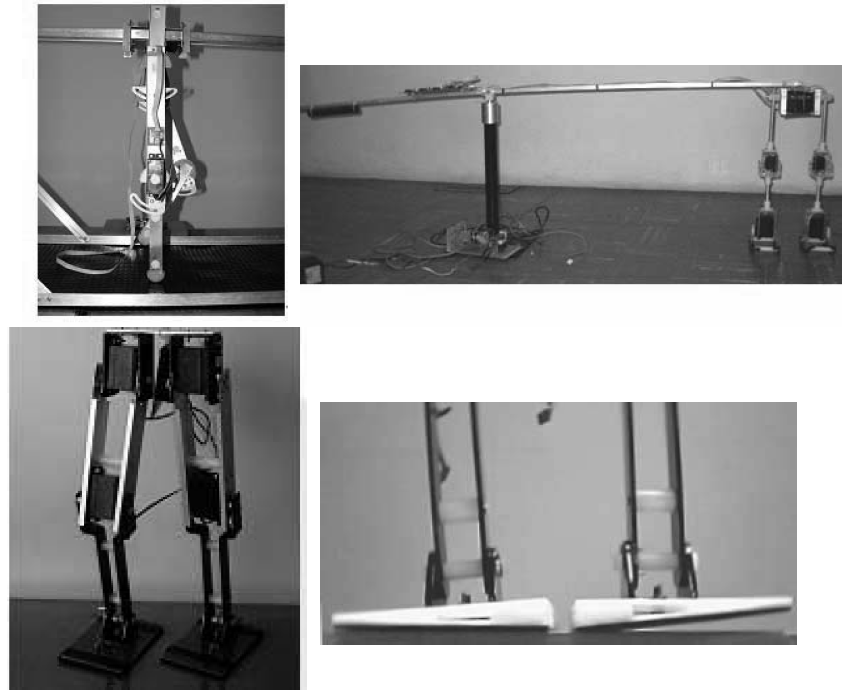
\includegraphics[scale=0.4]{../images/unroca.png}
  \caption{Robots serie UNROCA. [Tomado de \cite{M2005}]}
  \label{fig:unroca}
\end{figure}

\subsection{Algunas trabajos de investigaci\'on en la actualidad }
\label{sec:algtra}

\subsubsection{Generaci\'on de trayectorias y control}
\label{sec:gentray}
Simulaci\'on de un robot b\'ipedo empleando una m\'etodo evolutivo. 10 DOF y 7 eslabones, el m\'etodo PSO (Particle swarm optimization) asegura la estabilidad usando como restricci\'on el centro de masa CoM del pol\'igono de soporte\cite{Kherici2014}.\par
Se compara varios m\'etodos de optimizaci\'on multiobjetivo NSGAII, Sigma method, MOGA con el m\'etodo MOPSO. El m\'etodo es utilizado para sintonizar un controlador "robust sliding tracking". En el proceso se reduce una b\'usqueda heur\'istica de parámetros por ensayo-error, a una b\'usqueda \'optima seg\'un criterios de dise\'~no. Un operador de turbulencia es utilizado para evadir \'optimos locales\cite{Mahmoodabadi2014}.\par
Se proponen trayectorias \'optimas y din\'amicamente estables para subir y bajar escaleras basadas en el movimiento humano. Siete caracter\'isticas son resaltadas. Un algoritmo gen\'etico de c\'odigo real es utilizado para optimizar la marcha del robot y mejorar el consumo de energ\'ia y fortalecer la estabilidad. Simulaciones sobre configuraciones de 12-DOF son simuladas, basadas en las capturadas del movimiento humano durante el ascenso y el descenso de escaleras\cite{Lim2014}.\par
Se emplea un control (0-flat normal form) en una plataforma b\'ipeda de 7-DOF. Los resultados obtenidos muestran el buen desempe\~no de este m\'etodo para proponer leyes de control en sistemas altamente no-lineales. Adicional se propone una estrategia de dise\~no para controladores en robots caminadores\cite{Bououden2014}.\par
Se plantea un control compensado para evitar que perturbaciones externas, saquen de control el sistema. El sistema de aprendizaje mediante m\'aquinas de soporte vectorial difuso. Los resultados son comparados con otros m\'etodos inteligentes y se muestra su superioridad, mostrando una mayor sensibilidad y aumentando los rangos de estabilidad. En las fases de SSP y DSP se introducen conjunto de pertenencia de  triangulares y Gauss que permiten formular propiedades temporales de las marchas de robots con perturbaciones externas\cite{Wang2013}.\par
Usando el robot ePaddle, dise\~nado para actuar en medios terrestres, acu\'aticos y terrenos anfibios. Se estudia la marcha en modo carrera caminata. Simulaciones subiendo escaleras y siguiendo trayectorias circulares, muestran la estabilidad y eficiencia encontrada\cite{Sun2013}.\par
Generaci\'on en tiempo real de trayectorias para un robot de siete eslabones planar\cite{Farzaneh2014}.\par

\subsubsection{Biomec\'anica, Caminata,  Modelado y S\'intesis de mecanismos}
\label{sec:ascapa}
Un arreglo de sensores de fuerza flexible (FFSA) es construido para caracterizar el contacto del pie con terrenos irregulares, para determinar el área efectiva de contacto (ECA). Esta área es importante para mantener el balance dinámico y por lo tanto es utilizado en un esquema adicional de control para caminar sobre terrenos irregulares\cite{Wu2013}.\par
Una rodilla basada en mecanismos de cuatro barras es investigada en el desempe\~no de robots bípedos. Es comparada con la articulaci\'on tradicional rotacional de los robots. Concluyendo que aunque para bajas velocidades la articulaci\'on rotacional es mejor, en altas velocidades el mecanismo de cuatro barras muestra un mejor desempe\~no. El mecanismo de cuatro barras es optimizado siguiendo los ciclos de marcha óptimos\cite{Aoustin2013}.\par
Se dise\~na una rodilla (mediante optimizaci\'on perimétrica) basada en rodadura natural de la rodilla, se obtiene un mejoramiento en el consumo energético de los actuadores comparados con las rodillas de rotación tradicional\cite{Hobon2014}.\par
Modelado del efecto del contacto de rodadura de la planta del pie en la dinámica de caminar. El contacto es descrito por las longitudes del retropie, mediopie y antepie. Los parámetros anteriores son relacionado con los principales descriptores de marcha como la velocidad media , el periodo de paso en ángulo de entrepierna y la longitud de paso, así como la energía mecánica. Estas relaciones resultan útiles para el dise\~no de prótesis y la estabilidad del sistema\cite{Mahmoodi2013}.\par
Un nuevo dise\~no m\'as parecido a las características humanas en cuanto a la rodilla, el contacto de la planta del pie, inspirados en la forma del esqueleto humano, especialmente la pelvis. Las ventajas de la pelvis se ven reflejadas en el manejo del centro de gravedad de la parte superior del cuerpo humano. Un mejor modelo del pie conlleva a modelo de péndulo invertido durante sus fases\cite{Chiang2013}.\par
Basados en el modelo de la din\'amica de la caminata pasiva, específicamente la marcha del compás, la cual exhibe propiedades de caos. Se linealiza el modelo alrededor de un ciclo limite híbrido. Usando los mapas de Poincar\'e, es dise\~na un control por realimentaci\'on de estados, para convertir el sistema pasivo en activo\cite{Gritli2013}.\par
Se realiza el dise\~no de la lagartija Jesucristo, basado en un mecanismos Watt-I y los grupos de Assur. Se utiliza un algoritmo de control CPG(Central Pattern Generator) del sistema neural, para el balance y el ajusta de la marcha \cite{Xu2013}.\par
Análisis del modelo dinámico, estabilidad y consumo de energ\'ia eficiente de un robot con seis extremidades\cite{Roy2013}.\par

\section{Definici\'on del problema}
\label{sec:problema}
\subsection{Identificaci\'on}
Se observa un estancamiento en la aplicaci\'on de los conocimientos de la Universidad en el \'area de la rob\'otica b\'ipeda que sean integrados de forma funcional en este campo. Diferentes materias de pregrado y posgrado que reflejan dicho conocimiento como: Rob\'otica, Din\'amica de robots, Biom\'ecanica, T\'ecnicas de control, Identificaci\'on de sistemas, Optimizaci\'on, Control de robots, Control Robusto, Sistemas embebidos, Computaci\'on flexible, Computaci\'on gr\'afica y varias m\'as, deben ser integradas para abordar la soluci\'on de diversos problemas presentes en la caminata rob\'otica, como se reporta en todas las referencias citadas de este documento.\par
Una de las posibles causas por las que se haya detenido el avance de este campo es tal vez que el conocimiento requerido para ser integraci\'on proviene de distintas disciplinas.\par

\subsection{Formulaci\'on del problema}
El problema central a trabajar es: poder proponer, analizar e implementar en una plataforma b\'ipeda real y/o simulada, estrategias de control de caminata, control de direcci\'on, balance ante perturbaciones, generaci\'on y planeaci\'on de trayectorias, control de trote, control de saltos, implementaci\'on de agentes inteligentes, as\'i como dise\~nos que sean eficientes en el consumo de energ\'ia y que funcionen con los actuadores disponibles. Todos los problemas mencionados son de inter\'es mundial en cientos de laboratorio en el planeta.

\section{Metodolog\'ia}
\label{sec:metodo}
El siguiente proceso se implementar\'a como mecanismo de control y realimentación de la evoluci\'on de la investigaci\'on y el adecuado avance hacia sus objetivos, se repetir\'a a lo largo del desarrollo de la tesis, el cual se iterar\'a durante al menos cinco veces, (ver Fig.\ref{fig:method}, en donde se enumeran cada uno de los pasos).
\begin{figure}[!htb]
  \centering
  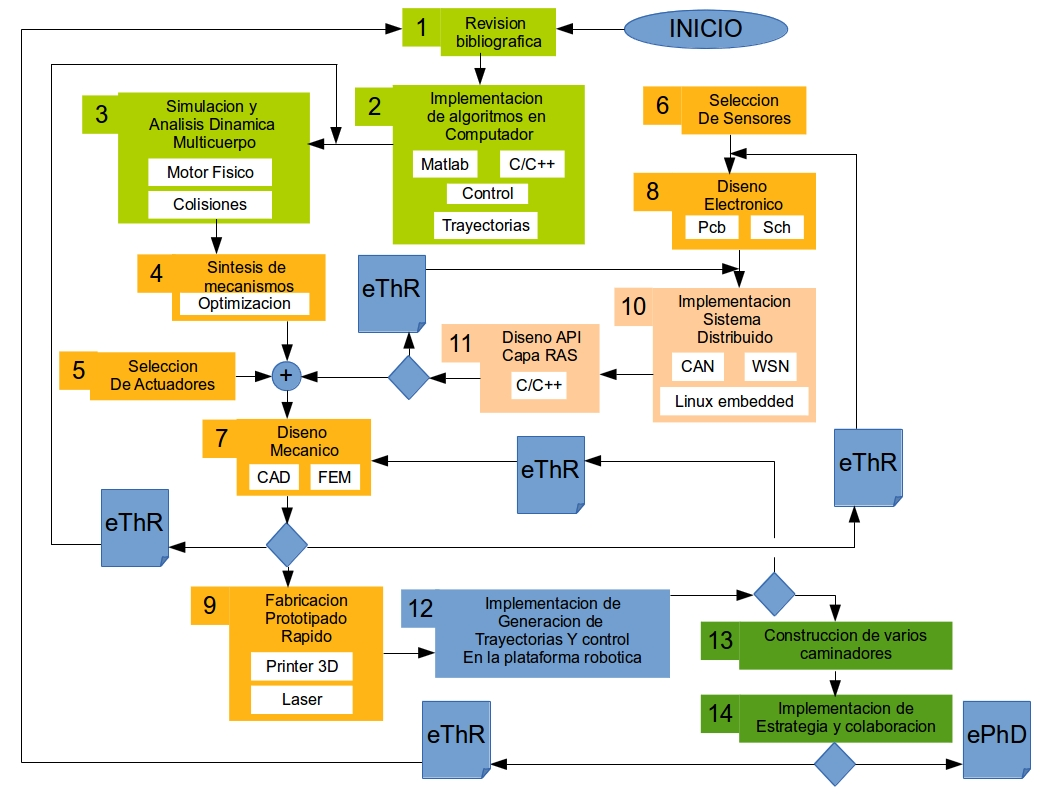
\includegraphics[scale=0.42]{../images/metGen2.png}
  \caption{Metodolog\'ia general}
  \label{fig:method}
\end{figure}
\begin{enumerate}[\textbf{Paso} 1:]
\item \textbf{Revisi\'on bibliogr\'afica -} Generar y ampliar continuamente un estado del arte sobre los temas relacionados, esto es consultar constantemente art\'iculos de revistas que se encuentren actu\'almente investigando sobre el tema. La constante actualizaci\'on del estado del arte serviar\'a para estar al tanto de nuevos avances en el tema. Continuar al \emph{paso 2}.\par
\item \textbf{Implementaci\'on computacional de algoritmos -} Se intentar\'a comprobar los resultados y consejos de los art\'iculos que sean m\'as relevantes para lograr los objetivos de la tesis. La implementaci\'on de algoritmos de control, generaci\'on de trayectoria y optimizaci\'on se realizar\'an utilizando una combinaci\'on de los lenguajes C/C++, Matlab, librer\'ias y toolboxes disponibles. En este paso es importante la seleci\'on, la generaci\'on y/o manejo de librer\'ias de mec\'anica multicuerpo. Librer\'ias como Cocos2d, Box2d, OGRE o Unity3d de uso libre y/o comercial, requieren ser analizadas en esta etapa. Continuar al \emph{paso 3}.\par
\item \textbf{Simulaci\'on y an\'alisis de la din\'amica multicuerpo - } Escogido un Framework para trabajar las necesidades requeridas para la implementaci\'on del paso 2, este paso tiene como objetivo analizar propuestas de dise\~no m\'ecanico, sugeridas por los pasos o iteraciones anteriores y probar los desempe\~nos de los algoritmos. En resumen modelar, simular, analizar y s\'intetizar mecanismos subactuados que optimicen la energ\'ia para la locomoci\'on de caminar, saltar o correr. Continuar al \emph{paso 4}.\par
\item \textbf{S\'intesis de mecanismos - } Utilizando t\'ecnicas bio-inspiradas, optimizaci\'on y algoritmos evolutivos, se har\'a una b\'usqueda de los parámetro de dise\~no que formar\'an las cadenas cinem\'aticas que propondrán una configuraci\'on b\'ipeda. Esta búsqueda optimizara el consumo de energ\'ia y tendrá en cuenta la forma de los actuadores. Continuar al \emph{paso 7}.\par
\item \textbf{Selecci\'on de actuadores - } Se deber\'a probar con distintos tipos de actuadores, motores de paso, servos, motores DC brushless, etc., que modificar\'an partes del dise\~no mecanico, en forma y en material. Etapas de potencia. Continuar al \emph{paso 7}.\par
\item \textbf{Selecci\'on de sensores - } Selecci\'on y prueba de IMUs, strain-gauges, reflectores de fuerza, sensores de temperatura, encoders, etc. Continuar al \emph{paso 8}.\par
\item \textbf{Dise\~no Mec\'anico - } El resultado de esta etapa debe ser un dise\~no robusto y en detalle de una plataforma modular capaz de configurar cadenas cinem\'aticas controladas y/o monitorizadas bajo el sistema distribuido. Adem\'as los disen\~os ser\'an basados en la caminata pasiva y el almacenamiento de energ\'ia mediante elementos pasivos que dejan como resultado los pasos anteriores. Si el dise\~no no es fabricable y el hilo de iteraci\'on es mec\'anico ir al \emph{paso 3} y escribir un reporte t\'ecnico, preparaci\'on para ponencias o congresos. Pero si el dise\~no no es fabricable y el hilo de iteraci\'on es electr\'onico ir al \emph{paso 8} si es fabricable ir al \emph{paso 9} y escribir un reporte t\'ecnico, preparaci\'on para ponencias o congresos.\par
\item \textbf{Dise\~no Electr\'onico - } Dise\~no de esquemas electrónicos, selección de ICs y fabricaci\'on de tarjetas (PCBs), para pruebas del sistema de la capa RAS. Continuar al \emph{paso 10}.\par
\item \textbf{Fabricaci\'on prototipo r\'apido - } Se construir\'a una plataforma rob\'otica modular y fabricada por prototipado, impresión 3D o corte por láser (ver Figura \ref{fig:objCapas} Capa Física). Continuar al \emph{paso 12}.\par
\item \textbf{Implementaci\'on del Sistema Distribuido - } Fabricaci\'on de PCBs de prototipo o definitivas, y pruebas sobre la red. Pruebas y manejo de CANbus, ZigBee y BLE. Definición de las tramas de comunicaci\'on. Continuar al \emph{paso 11}.\par
\item \textbf{Dise\~no API Capa RAS - } Implementar librerías en C/C++ que permita organizar la red de sensores y actuadores para que funciones en tiempo real organizando los procesos del sistema para que sean manejados por eventos o por temporizaci\'on por un controlador central con Linux embebido. Si se logra el requisito de tiempo-real continuar al \emph{paso 7}, si no ir al \emph{paso 10} y escribir un reporte t\'ecnico, preparaci\'on para ponencias o congresos.\par
\item \textbf{Implementación en la Plataforma Rob\'otica - } En esta etapa se prueban sobre la plataforma rob\'otica los algoritmos implementados en el computador en los pasos anteriores. Si el desempe\~no es el adecuado continuar al \emph{paso 13}, si no regresar a la etapa de dise\~no en el \emph{paso 7} y escribir un reporte t\'ecnico, preparaci\'on para ponencias o congresos.\par
\item \textbf{Construcción de varios prototipos - } Esta etapa despu\'es de probar que la plataforma construida funciona adecuadamente como agente individual, se construir\'an m\'as plataformas para que pueda interactuar entran a estudiar los agentes inteligentes en grupo. . Continuar al \emph{paso 14}.\par
\item \textbf{Implementaci\'on Agente Inteligente - } Aceptado un prototipo funcional de la plataforma hasta la capa de control se deberá  implementar estrategias y actividades colaborativas usando una red de caminadores  (ver Figura \ref{fig:objCapas} Capa Cognitiva.). Si se logra todos los objetivos finalizar escribiendo el documento final de la tesis, si no ir al \emph{paso 1} escribiendo un reporte t\'ecnico general de la iteraci\'on investigativa, preparaci\'on para ponencias o congresos.\par
\end{enumerate}
El tiempo que se tome en cada uno de los pasos anteriores ser\'a seg\'un se necesite, aunque inicialmente se dar\'a un tiempo limite seg\'un el cronograma del proyecto.\par

\section{Cronograma}
\label{sec:cronograma}
En la secci\'on anterior, cada paso tiene un nombre resaltado en negrita, a estos 14 nombres se le denominar\'an Actividades en la tabla a mostrada a continuaci\'on (\tablename  \ref{tab:crono} y \ref{tab:crono2}.). La tabla del cronograma muestra también como se piensa ejecutar la metodolog\'ia propuesta anterior.\par
\begin{table}[!htb]
  \centering
  \newcolumntype{G}{>{\columncolor[gray]{0.0}}c}
  \newcommand{\Bk}{\multicolumn{1}{G}{ }}
  \begin{tabular}{|p{3.0cm}||c|c|c|c|c|c|c|c|c|c|c|c|}\hline
    Actividades&\multicolumn{12}{|c|}{Bimestre}\\\hline\hline
    1er y  2do A\~no&1&2 &3  &4  &5  &6  &7  &8  &9  &10 &11 &12 \\\hline
    Actividad 1. &\Bk&   &   &   &   &\Bk&   &   &   &\Bk&   &   \\\hline
    Actividad 2. &\Bk&\Bk&   &   &\Bk&\Bk&   &\Bk&\Bk&\Bk&\Bk&\Bk\\\hline
    Actividad 3. &   &\Bk&   &   &\Bk&\Bk&   &\Bk&\Bk&\Bk&\Bk&\Bk\\\hline
    Actividad 4. &   &\Bk&   &   &   &\Bk&\Bk&\Bk&\Bk&\Bk&\Bk&\Bk\\\hline
    Actividad 5. &\Bk&   &   &\Bk&   &\Bk&   &   &   &\Bk&   &   \\\hline
    Actividad 6. &\Bk&   &   &\Bk&   &\Bk&   &   &   &\Bk&   &   \\\hline
    Actividad 7. &   &   &\Bk&\Bk&\Bk&   &\Bk&\Bk&\Bk&   &\Bk&\Bk\\\hline
    Actividad 8. &   &\Bk&   &\Bk&   &\Bk&   &   &   &\Bk&   &   \\\hline
    Actividad 9. &   &   &   &\Bk&   &   &\Bk&\Bk&\Bk&   &\Bk&\Bk\\\hline
    Actividad 10.&   &   &\Bk&\Bk&\Bk&   &\Bk&\Bk&\Bk&   &\Bk&\Bk\\\hline
    Actividad 11.&   &   &\Bk&\Bk&\Bk&   &\Bk&\Bk&\Bk&   &\Bk&\Bk\\\hline
    Actividad 12.&   &   &   &   &\Bk&   &   &\Bk&\Bk&   &\Bk&\Bk\\\hline
    Actividad 13.&   &   &   &   &   &   &   &   &   &   &   &   \\\hline
    Actividad 14.&   &   &   &   &   &   &   &   &   &   &   &   \\\hline
    Escribir Doc &   &\Bk&   &\Bk&   &\Bk&   &\Bk&   &\Bk&   &\Bk\\\hline    
  \end{tabular}
  \caption{Cronograma de investigaci\'on de los primeros dos a\~nos}
  \label{tab:crono}
\end{table}
\begin{table}[!htb]
  \centering
  \newcolumntype{G}{>{\columncolor[gray]{0.0}}c}
  \newcommand{\Bk}{\multicolumn{1}{|G|}{ }}
  \begin{tabular}{|p{3.0cm}||c|c|c|c|c|c|c|c|c|c|c|c|}\hline
    Actividades&\multicolumn{12}{|c|}{Bimestre}\\\hline\hline
    %3er y  4to A\~no &13 &14 &15 &16 &17 &18 &19 &20 &21 &22 &23 &24 \\\hline
    1er y  2do A\~no&1&2 &3  &4  &5  &6  &7  &8  &9  &10 &11 &12 \\\hline
    Actividad 1. &\Bk&   &   &   &   &   &   &   &   &   &   &   \\\hline
    Actividad 2. &\Bk&\Bk&\Bk&\Bk&\Bk&\Bk&\Bk&   &   &\Bk&\Bk&   \\\hline
    Actividad 3. &\Bk&\Bk&\Bk&\Bk&\Bk&\Bk&\Bk&   &   &\Bk&\Bk&   \\\hline
    Actividad 4. &\Bk&   &   &   &   &   &   &   &   &   &   &   \\\hline
    Actividad 5. &   &   &   &   &   &   &   &   &   &   &   &   \\\hline
    Actividad 6. &   &   &   &   &\Bk&   &   &   &   &   &   &   \\\hline
    Actividad 7. &\Bk&   &   &\Bk&\Bk&   &   &   &   &   &   &   \\\hline
    Actividad 8. &   &   &   &   &   &   &   &   &   &   &   &   \\\hline
    Actividad 9. &\Bk&   &   &\Bk&\Bk&   &   &\Bk&\Bk&   &   &   \\\hline
    Actividad 10.&   &   &   &   &   &   &\Bk&   &   &   &\Bk&   \\\hline
    Actividad 11.&\Bk&   &   &   &   &   &\Bk&   &   &   &\Bk&   \\\hline
    Actividad 12.&\Bk&\Bk&\Bk&\Bk&\Bk&\Bk&\Bk&\Bk&\Bk&\Bk&\Bk&\Bk\\\hline
    Actividad 13.&   &   &   &\Bk&\Bk&   &   &\Bk&   &   &   &   \\\hline
    Actividad 14.&   &   &   &   &\Bk&\Bk&\Bk&   &\Bk&\Bk&\Bk&\Bk\\\hline
    Escribir Doc &   &\Bk&   &\Bk&   &\Bk&   &\Bk&   &\Bk&\Bk&\Bk\\\hline    
  \end{tabular}
  \caption{Cronograma de investigaci\'on de los dos \'ultimos a\~nos}
  \label{tab:crono2}
\end{table}

\section{Sectores de impacto}
\label{sec:impacto}
Aplicaci\'on de los conocimientos que se obtengan servir\'an en: 
\begin{itemize}
\item La industria de los manipuladores en el \'area de la teleoperaci\'on, como el robot Justin del DRL o el Robonout de GM.
\item La manufactura en el transporte de materiales y ensambles.
\item Los robots de servicio.
\item La fabricaci\'on de prótesis, dise\~no y optimizaci\'on.
\item La fisioterapia, sistemas de recuperaci\'on de lesiones o estimulaci\'on de movimiento.
\item La educaci\'on como herramienta did\'actica y motivacional.
\item El entretenimiento,el área de la teor\'ia de juegos y agentes inteligentes como es el caso del fútbol de robots.
\end{itemize}

\bibliographystyle{plain}
\bibliography{refsprop}
%\nocite{*}
\vspace{2cm}

\section*{Firmas:}
\label{firmas}
\vspace{4cm}
\parbox[b][3cm][c]{8cm}{
\centering
\rule{7cm}{1pt}\par
\textbf{Proponente:}\par
Jaime Andr\'es Castillo Le\'on
}\par\vspace{3cm}
\parbox[b][3cm][c]{8cm}{
\centering
\rule{7cm}{1pt}\par
\textbf{Director de investigaci\'on:}\par
PhD. Ing. Ricardo Ram\'irez Heredia
}

\end{document}
